\clearpage
\section{بخش سوم: ریاضیات کانولوشن (\lr{Convolution Mathematics})}

\begin{stepbox}
\field{پیاده‌سازی دستی کانولوشن و تکنیک \lr{im2col}}{
در این بخش، عملیات کانولوشن دوبعدی ابتدا به صورت دستی با استفاده از پنجره لغزان (\lr{Sliding Window}) و سپس با استفاده از الگوریتم پیشرفته‌ی (\lr{im2col}) پیاده‌سازی شده است تا عملیات کانولوشن به یک ضرب ماتریسی (\lr{Matrix Multiplication}) بهینه تبدیل شود.
}
\end{stepbox}

\begin{codebox}[پیاده‌سازی کانولوشن دستی و روش بهینه‌ی \lr{im2col}]
\begin{lstlisting}[language=Python]
# 1. روش پنجره لغزان (Sliding Window)
def manual_convolution(image, kernel):
    img_h, img_w = image.shape
    k_h, k_w = kernel.shape
    out_h, out_w = img_h - k_h + 1, img_w - k_w + 1
    output = np.zeros((out_h, out_w))
    for i in range(out_h):
        for j in range(out_w):
            patch = image[i:i+k_h, j:j+k_w]
            output[i, j] = np.sum(patch * kernel)
    return output

# 2. روش بهینه im2col (تبدیل به ضرب ماتریسی)
def im2col_convolution(image, kernel):
    img_h, img_w = image.shape
    k_h, k_w = kernel.shape
    out_h, out_w = img_h - k_h + 1, img_w - k_w + 1
    X_col = np.zeros((out_h * out_w, k_h * k_w))
    row_idx = 0
    for i in range(out_h):
        for j in range(out_w):
            X_col[row_idx, :] = image[i:i+k_h, j:j+k_w].flatten()
            row_idx += 1
    out_flat = X_col @ kernel.flatten()
    return out_flat.reshape((out_h, out_w))
\end{lstlisting}
\end{codebox}

\subsection{اعمال فیلترهای فضایی و ارزیابی خروجی‌ها}

در ادامه، سه فیلتر پایه شامل فیلتر لبه‌یاب (\lr{Sobel})، فیلتر تارکننده (\lr{Blur}) و فیلتر تیزکننده (\lr{Sharpen}) بر روی تصویر اعمال گردیده‌اند.

\begin{figure}[htbp]
    \centering
    \begin{subfigure}{0.32\textwidth}
        \centering
        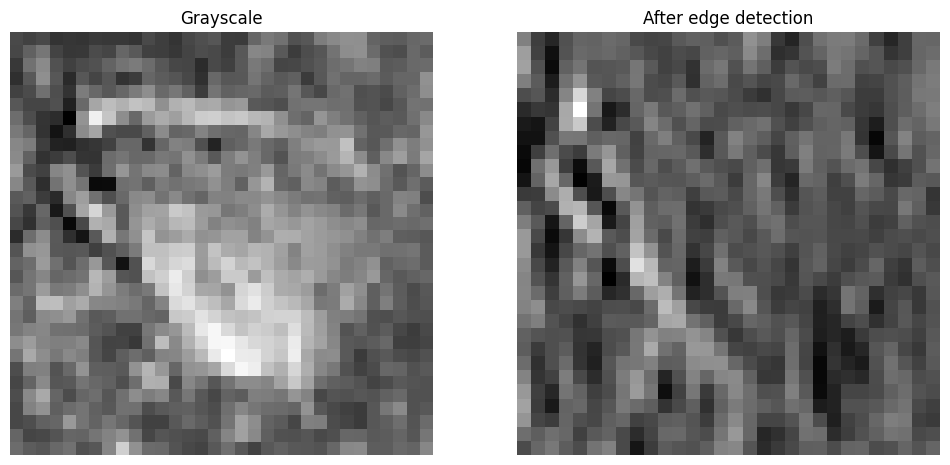
\includegraphics[width=\textwidth]{images/img_conv_edge.png}
        \caption{فیلتر لبه‌یاب (\lr{Edge Detection})}
    \end{subfigure}
    \hfill
    \begin{subfigure}{0.32\textwidth}
        \centering
        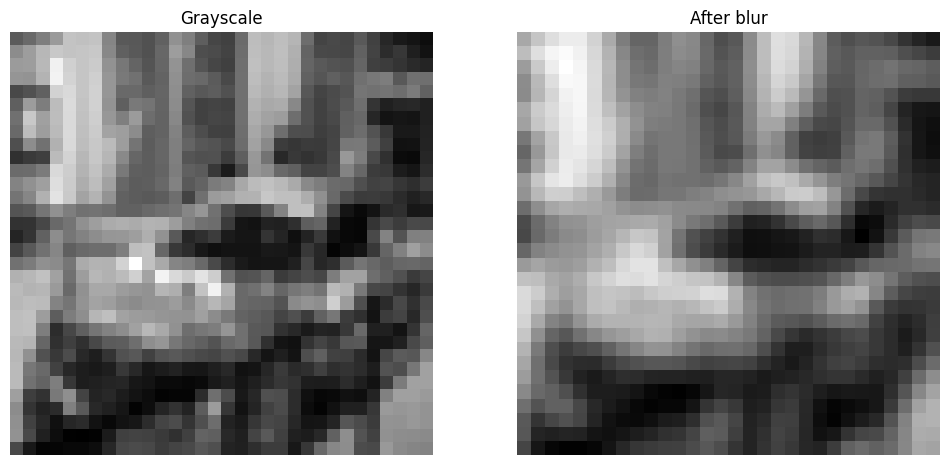
\includegraphics[width=\textwidth]{images/img_conv_blur.png}
        \caption{فیلتر تارکننده (\lr{Blur})}
    \end{subfigure}
    \hfill
    \begin{subfigure}{0.32\textwidth}
        \centering
        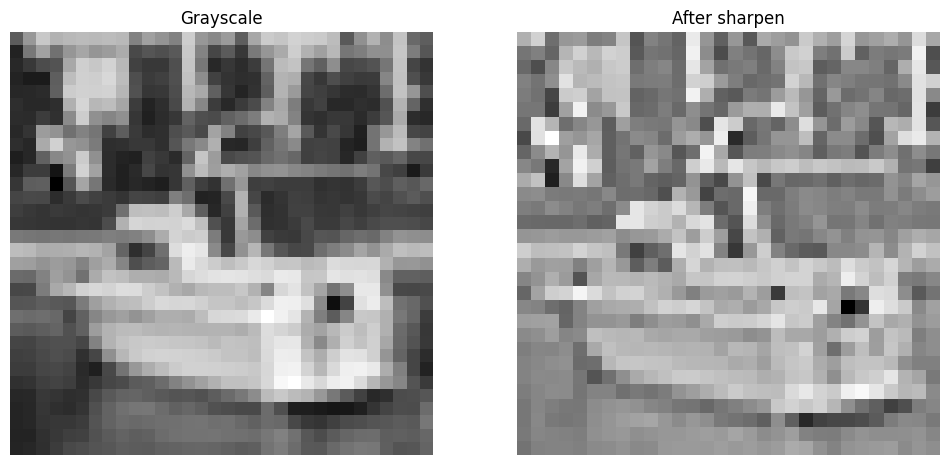
\includegraphics[width=\textwidth]{images/img_conv_sharpen.png}
        \caption{فیلتر تیزکننده (\lr{Sharpen})}
    \end{subfigure}
    \caption{نمایش اثر فیلترهای مختلف بر روی تصویر ورودی}
    \label{fig:filters_grid}
\end{figure}

\begin{stepbox}
\field{تحلیل ریاضی عملکرد کرنل‌ها}{
\textbf{۱. فیلتر لبه‌یاب (\lr{Edge Detection}):} \\
کرنل لبه‌یاب با محاسبه‌ی مشتق تقریبی مکانی ($\nabla I$), اختلاف شدت روشنایی را سنجش می‌کند. در مناطق یکدست حاصل‌ضرب صفر شده و در مرزها به دلیل نرخ تغییرات بالا، مقادیر عددی بزرگی تولید می‌شود.

\textbf{۲. فیلتر تارکننده (\lr{Blur Kernel}):} \\
این کرنل مقادیر یکسانی با مجموع ۱ دارد (مانند ماتریس $3 \times 3$ با درایه‌های $\frac{1}{9}$). اثر ریاضی آن میانگین‌گیری موضعی (\lr{Low-pass Filter}) است که فرکانس‌های بالا (جزئیات و نویزها) را تضعیف کرده و تصویر را هموار می‌سازد.

\textbf{۳. فیلتر تیزکننده (\lr{Sharpen Kernel}):} \\
این فیلتر با تخصیص وزن مثبت بالا به پیکسل مرکزی و وزن‌های منفی به پیکسل‌های مجاور، اختلافات محلی را تشدید می‌کند (\lr{High-pass Filter}) که منجر به برجسته‌تر شدن لبه‌ها و جزئیات بافت می‌شود.
}
\end{stepbox}

\subsection{ارزیابی سرعت و صحت روش \lr{im2col}}

\begin{figure}[htbp]
    \centering
    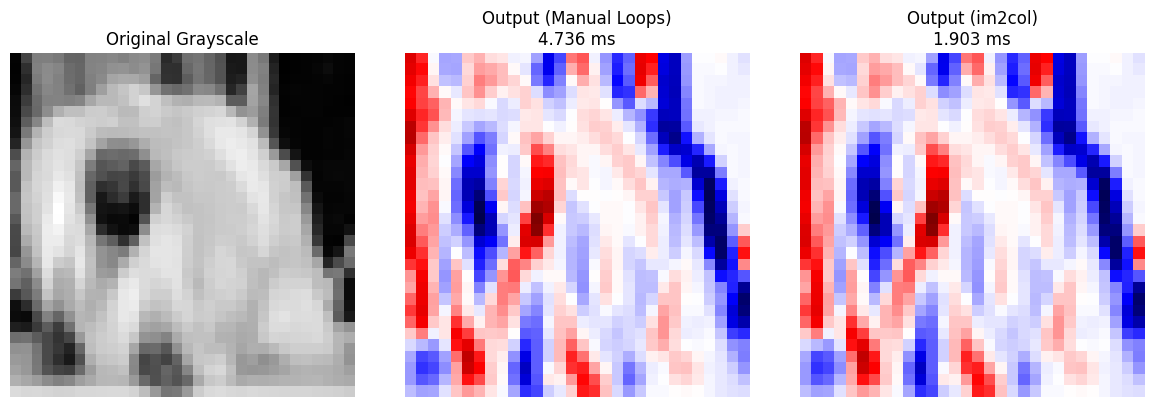
\includegraphics[width=0.88\textwidth]{images/img_conv_speed_comparison.png}
    \caption{مقایسه زمان اجرا و یکسانی ریاضی خروجی حلقه‌های دستی (\lr{Manual Loop}) و الگوریتم (\lr{im2col})}
    \label{fig:speed_comp}
\end{figure}

\begin{tipbox}[مزیت محاسباتی \lr{im2col}]
الگوریتم (\lr{im2col}) با استخراج وصله‌ها و تبدیل آن‌ها به سطر‌های ماتریس $X_{col}$ با ابعاد $(N_{patches} \times K_{size})$، عملیات کانولوشن را به یک ضرب ماتریسی ($X_{col} \cdot K_{flat}$) تبدیل می‌کند. این ساختار امکان بهره‌گیری از هسته‌های پردازش موازی در (\lr{GPU}) و کتابخانه‌های بهینه‌ی جبر خطی (\lr{BLAS}) را فراهم کرده و زمان محاسبات را به شدت کاهش می‌دهد.
\end{tipbox}